%\begin{figure}
\begin{center}
\tikzstyle{hidden}=[circle,
                        thick,
                        draw=black,
                        fill=white]
                        % minimum size=1.5ex,


\tikzstyle{observed}=[circle,
                        thick,
                        draw=black,
                        fill=gray!60]
                        % minimum size=1.5ex,


\tikzstyle{plate}=[rectangle,
                        draw=black,
                        fill=none,
                        inner sep=.8ex,
                        rounded corners=.6ex]

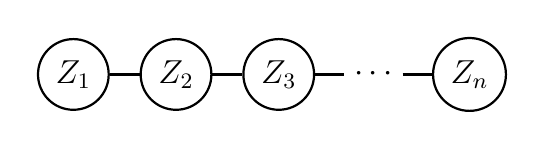
\begin{tikzpicture}[>=latex] %,text height=1.5ex,text depth=0.25ex]
  % The various elements are conveniently placed using a matrix:
  \matrix[row sep=2.5ex,column sep=2.5ex] {
        \node (Z1) [hidden] {\large $Z_1$};  & 
        \node (Z2) [hidden] {\large $Z_2$};  & 
        \node (Z3) [hidden] {\large $Z_3$};  & 
        \node (dots) {\large $\cdots$};  & 
        \node (Zn) [hidden] {\large $Z_n$};
		\\
    };
    
    % The diagram elements are now connected through arrows:
    \path[-]
        (Z1) edge[thick] (Z2)
        (Z2) edge[thick] (Z3)
        (Z3) edge[thick] (dots)
        (dots) edge[thick] (Zn)
;
        
\end{tikzpicture}
\end{center}
%\caption{}
%\end{figure}